\documentclass[12pt]{article}

% --- Packages ---
\usepackage[margin=1in]{geometry}
\usepackage{amsmath,amssymb,amsthm}
\usepackage{booktabs}
\usepackage{graphicx}
\usepackage{natbib}
\usepackage{hyperref}
\usepackage{setspace}
\usepackage{enumitem}
\usepackage{caption}
\usepackage{float}
\usepackage[most]{tcolorbox}
\usepackage{colortbl}

\setstretch{1.5}

% --- Theorem environments ---
\newtheorem{proposition}{Proposition}
\newtheorem{corollary}{Corollary}
\newtheorem{lemma}{Lemma}
\theoremstyle{definition}
\newtheorem{definition}{Definition}
\newtheorem{assumption}{Assumption}
% Remark as a shaded box with rounded edges
\newtcolorbox{remark}[1][]{
  colback=gray!8,
  colframe=gray!40,
  arc=3pt,
  boxrule=0.5pt,
  left=8pt, right=8pt, top=6pt, bottom=6pt,
  fonttitle=\bfseries,
  title={Remark\ifx&#1& \else: #1\fi},
}

% --- Title ---
\title{\textbf{Against the Coasean Singularity}\\ \large Conditions for a Conglomerate Premium in AI-Era Industrial Organization}
\author{Soren Larson\thanks{Correspondence: \texttt{@hypersoren}. The author thanks Byrne Hobart (\texttt{@ByrneHobart}) for early intellectual contributions to the rollup framing, and Jeremy Giffon (\texttt{@jeremygiffon}) for crystallizing the scale-margin thesis. Computational results and replication code are available at \url{https://github.com/sorenlarson/against-coasean-singularity}.}}
\date{March 2026}

\begin{document}

\maketitle

\begin{abstract}
\begin{spacing}{1.2}
\noindent AI commoditizes execution, so value migrates to the inputs execution cannot replace: local context, trust, and operational control. A growing literature argues that AI agents will reduce transaction costs enough to shift activity from firms to markets---a ``Coasean singularity.'' We argue that coordination requires \textit{context revelation}, which leaks the scarce resource that generates value. Who owns the assets where context is born determines who captures that value. We develop a framework that maps the parameter space of information economics---leakage persistence, context specificity, cross-node transferability---to institutional form dominance across four regimes: fragmented market, platform router, data-isolated router, and vertically integrated rollup. The framework identifies three mechanisms driving ownership advantage, in stable rank order: router learning leakage (the systematic redistribution of client operational intelligence), cross-node learning transfer, and leakage protection. Channel rankings hold across calibrations and graph sizes; magnitudes are calibration-dependent. We calibrate the framework to 35 AI-native services verticals and generate testable predictions: the ownership advantage is largest where context is persistent (leaked information stays exploitable for a long time) and specific (revealing it destroys competitive value)---cybersecurity, accounting, insurance brokerage---and smallest where context is ephemeral and commoditized---IT services, travel, admin. A data-isolated router---the platform's best response---eliminates the dominant channel but cannot replicate the ownership-contingent channels, trailing the rollup under every tested calibration. In competing-world simulation with preemptive data isolation (the router's strongest strategy, applied from step 0), competitive feedback still compounds the structural advantage: the rollup wins across all tested seeds.

\bigskip
\noindent \textit{JEL Codes:} D23, L22, L25, O33 \\
\textit{Keywords:} Theory of the firm, transaction costs, artificial intelligence, vertical integration, platform economics, roll-ups
\end{spacing}
\end{abstract}

\newpage
\tableofcontents
\newpage

%=============================================================================
\section{Introduction}
%=============================================================================

Competitive advantage in a market economy comes from the abundant provision of scarce goods.\footnote{This formulation draws on \citet{danco2017}, who argues that scarcity reappears elsewhere when technology removes friction. See also \citet{christensen1997} on the conservation of attractive profits.} When a production input becomes commoditized, value migrates to whatever remains scarce. AI is commoditizing execution---the cognitive work of search, negotiation, monitoring, and coordination that previously required expensive human judgment. As execution becomes cheap, scarcity flees to the inputs that execution cannot replace: \textit{local context}, \textit{trust}, and \textit{operational control}.

The standard account runs as follows: AI reduces transaction costs, making it cheaper to coordinate across firm boundaries, which should---following \citet{coase1937}---shrink the optimal firm and expand market coordination. In the limit, firms dissolve into networks of autonomous AI agents: the ``Coasean singularity'' \citep{shahidi2025}. This view has broad support.\footnote{Google DeepMind proposes ``sandbox economies'' where autonomous agents transact at speeds beyond human oversight \citep{tomasev2025}; technology analysts project 60 billion agents within a decade \citep{azhar2024}; MIT researchers propose ``protocol-centric intelligence'' as a replacement for firm-based coordination \citep{chopra2024}.} But if value has migrated to context, trust, and control, then the question is not how cheaply agents can process information across boundaries. It is who \textit{owns} the scarce inputs---and what happens to those inputs when they cross a boundary. Context degrades when it is shared: revealing private information to coordinate with a counterparty creates \textit{leakage} that erodes the scarcity that made the information valuable. The severity depends on institutional form.

The argument turns on four observations:

\begin{enumerate}[leftmargin=*]
\item \textbf{Context revelation creates leakage.} To coordinate, a firm must reveal private context: demand signals, pricing sensitivity, capacity constraints. Once revealed, this information leaks to the broader market. The severity depends on institutional form.

\item \textbf{Learning compounds under common ownership.} When multiple nodes share an owner, successful coordination at one node generates learning signals that transfer to others, creating a policy quality flywheel.

\item \textbf{Ownership forecloses competitors' access.} Acquiring a node removes it from the router's client base, reducing the router's coordination opportunities and learning breadth. The Shapley-decomposed contribution of context blurring is near zero ($-0.006$), but node removal drives the tipping dynamic.

\item \textbf{Trust is the router's advantage, not the rollup's.} The router must \textit{earn} trust through investment; the rollup accesses context through \textit{ownership}. When trust is removed from the model, the router loses its main differentiator while the rollup barely notices.
\end{enumerate}

We formalize these observations in a directed-graph model where nodes are firms, edges are coordination relationships, and four institutional forms are evaluated over the same graph. The four forms correspond to competing theses about AI-era industrial organization: the \textbf{market} (Coasean singularity), the \textbf{router} (SaaS platform), the \textbf{data-isolated router} (platform's best response, contractually preventing cross-client data use), and the \textbf{rollup} (cybernetic rollup thesis, \citet{larson2025cybernetic, hobart2024routers}).

Our main findings are:

\begin{enumerate}[leftmargin=*]
\item \textbf{A conglomerate premium emerges from structure alone.} Portfolio value exceeds the sum of parts without assumed complementarity---contradicting the well-documented conglomerate discount \citep{berger1995}. The premium has two components: each additional node creates new coordination opportunities with every existing node (a network-size effect), and common ownership makes those opportunities more valuable per interaction than they would be under separate ownership (the ownership-specific effect from internal visibility and cross-node learning).

\item \textbf{Three mechanisms} drive the premium, in stable rank order: router learning leakage ($\sim$66\%), cross-node learning transfer ($\sim$23\%), and leakage protection ($\sim$16\%). Rankings hold across calibrations; magnitudes are calibration-dependent.

\item \textbf{Industry calibrations}: the advantage is largest where context is persistent and specific, smallest where it expires quickly and carries little competitive value. We calibrate 35 AI-native services verticals.

\item \textbf{A data-isolated router}---the platform's best response---eliminates the dominant channel but still loses to the rollup by $\sim$12\%.

\item In \textbf{competing-world simulation}, competitive feedback compounds the advantage ($\sim$1.9$\times$ the router's surplus), surviving preemptive data isolation from step 0.
\end{enumerate}

The paper contributes to the theory of the firm \citep{coase1937, williamson1975, grossman1986, hart1990} by identifying cross-node learning transfer under common ownership as a mechanism distinct from classical hold-up or residual control rights; to platform economics \citep{rochet2003, parker2016} by formalizing conditions under which ownership dominates intermediation; and to AI and industrial organization \citep{agrawal2018, brynjolfsson2017} by providing testable predictions about consolidation versus fragmentation.\footnote{\textbf{Related literature.} \citet{coase1937} showed firms exist to economize on transaction costs; \citet{williamson1975, williamson1985} identified asset specificity as the key determinant of governance structure; \citet{grossman1986} and \citet{hart1990} reframed ownership as conferring residual control rights under incomplete contracts. Our model departs from these frameworks: ownership changes the \textit{information topology}---preventing leakage, accelerating learning, and foreclosing context---rather than reducing costs. In platform economics, \citet{rochet2003} and \citet{armstrong2006} developed two-sided platform theory; our router regime operationalizes their assumption that intermediation suffices, and shows its structural ceiling. On conglomerates, the diversification discount \citep{berger1995, lang1994, jensen1986} predicts that combining businesses destroys value; our model identifies conditions (AI-enabled cross-node learning with leakage-sensitive context) under which a conglomerate \textit{premium} emerges. \citet{shahidi2025} provide the most comprehensive articulation of the market-expansion thesis, treating agents as autonomous market participants that reduce transaction costs; our model identifies three gaps: context revelation creates leakage their framework does not account for, trust-generated context only exists in trusted interactions (not a search cost problem), and the critical ownership question is who owns the \textit{asset where context is born}, not who owns the agent. \citet{bonatti2022} show that information monopolists facing competing buyers maximize revenue through \textit{exclusive} provision---the foreclosure mechanism in our simulation is the structural analogue of this exclusivity result.}

%=============================================================================
\section{Model}
%=============================================================================

Consider a directed graph economy $\mathcal{G} = (\mathcal{V}, \mathcal{E})$ with $N = |\mathcal{V}|$ nodes (firms) and edges representing potential coordination relationships. Time is discrete: $t \in \{1, \ldots, T\}$. Nodes are partitioned into $K$ verticals. Each node $i$ is characterized by a vertical assignment $v_i$, context vectors $\mathbf{d}_i, \mathbf{c}_j \in [0,1]^7$ (demand and capacity profiles for computing coordination fit), hidden alpha $\alpha_i \in [0,1]$ (private information value), actuator strength $a_i$, exception rate $\xi_i$, and quality risk $\omega_i$. Each edge $(i,j)$ carries a base surplus $s_{ij}$, leakage sensitivity $\ell_{ij}$, trust requirement $\tau_{ij}$, complementarity $\kappa_{ij}$ (set to zero by default), latency cost $\lambda_{ij}$, and execution risk $\epsilon_{ij}$.

Three institutional forms are evaluated over the same graph in a parallel-world design: the same economy is run separately under each form, cleanly attributing performance differences to institutional structure.\footnote{A competing-world extension where the four forms coexist and compete is presented in Section~\ref{sec:competing}.} Each form is characterized by three parameters: visibility $\nu_{ij}$ (how much of what you reveal ends up visible to competitors---low for internal rollup interactions, high in the open market), actuator multiplier $\mu_{ij}$ (whether you can act on what you learn or only recommend---full control for rollup-owned pairs, advisory-only otherwise), and interaction mode $\iota_{ij}$ (how readily the relationship surfaces sensitive context---high for owned subsidiaries, moderate for platform clients, low for arm's-length transactions). Let $\mathcal{O}^t \subseteq \mathcal{V}$ denote the set of nodes owned by the rollup at time $t$.

\begin{table}[H]
\centering
\caption{Institutional Form Parameters}
\label{tab:params}
\begin{tabular}{lcccc}
\toprule
Parameter & Market & Router & Iso.\ Router & Rollup \\
\midrule
Visibility $\nu_{ij}$ & 1.0 & 0.85 & 0.85 & $\begin{cases} 0.1 & i,j \in \mathcal{O}^t \\ 0.85 & \text{else} \end{cases}$ \\[8pt]
Actuator $\mu_{ij}$ & 0.5 & 0.5 & 0.5 & $\begin{cases} 1.0 & i,j \in \mathcal{O}^t \\ 0.5 & \text{else} \end{cases}$ \\[8pt]
Interaction $\iota_{ij}$ & 0.2 & 0.6 & 0.6 & $\begin{cases} 1.0 & i,j \in \mathcal{O}^t \\ 0.2 & \text{else} \end{cases}$ \\[8pt]
Learning leakage $\lambda_R$ & 0 & 0.15 & 0 & 0 \\
Base learning rate & 0.03 & 0.03 & 0.03 & 0.03 \\
Signal quality $\sigma_q$\textsuperscript{a} & 0.3 & $0.5 + \text{b.}$\textsuperscript{b} & $0.5 + \text{b.}$\textsuperscript{b} & wt.\ avg\textsuperscript{c} \\
Transfer bonus\textsuperscript{d} & 0 & 0 & 0 & $\tau \cdot |\{v_k\}| / K$ \\
Per-step cost & 0 & 0 & $c_{\text{sub}} \cdot N$ & $c_{\text{own}} \cdot |\mathcal{O}^t| + \sum f_j^t$ \\
\bottomrule
\end{tabular}

\vspace{4pt}
\begin{spacing}{1.0}
{\small
\textsuperscript{a}Signal quality determines how much of a coordination outcome's information content each regime can observe, modulating the effective learning rate.

\textsuperscript{b}The router's signal quality includes a breadth bonus from observing all client interactions: $0.5 + \ln(1 + |\mathcal{E}^t_R|)/10$, reflecting how platforms like Stripe learn from aggregate transaction patterns.

\textsuperscript{c}The rollup's signal quality is a weighted average of internal ($\sigma_{\text{own}} = 0.9$, full outcome observability) and external ($\sigma_{\text{mkt}} = 0.3$, price/quantity only), weighted by the fraction of events in each category.

\textsuperscript{d}Transfer bonus: cross-vertical learning available only to the rollup. Proportional to the number of distinct verticals represented in the owned portfolio ($|\{v_k\}|$) divided by total verticals ($K$). A rollup owning logistics and healthcare nodes learns faster than one concentrated in a single vertical, because operational patterns transfer across domains.
}
\end{spacing}
\end{table}

The data-isolated router has identical interaction parameters to the standard router but sets $\lambda_R = 0$: it contractually prevents cross-client data use, charging a subscription fee ($c_{\text{sub}}$) instead. This isolates the effect of learning leakage.

\subsection{Coordination Game}

At each time step, each node generates coordination opportunities (Poisson rate $\lambda_O$), selects a counterparty $j$, and chooses a revelation level $r \in [0,1]$ representing the fraction of private context disclosed. Match quality $m_{ij}(r) = \sigma(z_{ij})$ aggregates the channels through which coordination quality is determined:

\begin{equation}
\label{eq:match}
z_{ij} = \underbrace{\beta_0}_{\text{baseline}} + \underbrace{\beta_1 \ln(1 + b_r \cdot r)}_{\text{revelation}} + \underbrace{\beta_2 \cdot \hat{\tau}_{ij}}_{\text{trust context}} + \underbrace{\beta_3 \cdot q}_{\text{policy quality}} + \underbrace{\beta_4 \cdot \hat{a}_{ij}}_{\text{actuator}} + \underbrace{\beta_5 \cdot \kappa_{ij}}_{\text{complementarity}} + \underbrace{\beta_6 \cdot \phi_{ij}}_{\text{context fit}}
\end{equation}

\noindent The logarithmic revelation term ensures diminishing returns. Policy quality $q$ is accumulated institutional knowledge starting at 0.1 and improving through learning. Context fit $\phi_{ij} = \mathbf{d}_i \cdot \mathbf{c}_j / (\|\mathbf{d}_i\| \|\mathbf{c}_j\|)$ measures demand-capacity alignment. Trust-generated context $\hat{\tau}_{ij}$ is information that only exists because a trusted interaction occurred---not preexisting information that gets disclosed, but new information created by the quality of the interaction channel, scaling with pairwise trust, interaction mode, and available information.

Revelation creates leakage governed by a scale parameter $\lambda_L = 2.5$ and convexity exponent $\gamma = 1.5$:

\begin{equation}
\label{eq:leakage}
L_{ij}(r) = \underbrace{\lambda_L}_{\text{scale}} \cdot \underbrace{r^{\gamma}}_{\substack{\text{convex in} \\ \text{revelation}}} \cdot \underbrace{\ell_{ij}}_{\substack{\text{edge} \\ \text{sensitivity}}} \cdot \underbrace{\alpha_i}_{\substack{\text{info} \\ \text{value}}} \cdot \underbrace{\nu_{ij}}_{\substack{\text{market} \\ \text{visibility}}}
\end{equation}

\noindent Leakage is the product of how much you reveal ($r^\gamma$), how exploitable this edge is ($\ell_{ij}$), how valuable your information is ($\alpha_i$), and how exposed your interaction is ($\nu_{ij}$, varying by form per Table~\ref{tab:params}). Leakage accumulates in a persistent stock $S_i^t$ with decay rate $\rho = 0.8$. The router incurs additional \textit{router learning leakage} $L^R_{ij} = \lambda_R \cdot m_{ij} \cdot s_{ij}$, proportional to match quality and base surplus---better coordination reveals more operationally valuable information to be redistributed across all clients.

Net surplus from a coordination event is gross value minus latency cost (friction and delay, constant per edge), leakage cost, and execution loss: $\Pi_{ij}(r) = s_{ij} \cdot m_{ij}(r) - \lambda_{ij} - C_L(r) - X_{ij}$. Each node chooses $r^*_{ij} = \arg\max_r \Pi_{ij}(r)$.\footnote{The first-order condition equates marginal benefit of revelation (better match quality) with marginal cost (more leakage). By the implicit function theorem, optimal revelation is decreasing in visibility $\nu_{ij}$ and leakage sensitivity $\ell_{ij}$, and increasing in base surplus $s_{ij}$. Under baseline calibration, market and router nodes choose partial revelation in $\sim$19--20\% of events; the rollup reveals almost fully ($r = 1.00$ in 88\% of events) because its institutional form shields context.}

\subsection{Dynamics}

Pairwise trust $T_{ij}^t$ builds with successful coordination (rate $\eta^+ = 0.08$) and decays on failure ($\eta^- = 0.04$), with an ownership bonus ($b = 1.2$ for owned pairs). Each regime accumulates policy quality $q^t$ through learning, with the same base learning rate ($\eta_{\text{base}} = 0.03$) modulated by signal quality $\sigma_q$---how much of each coordination outcome's information content the regime can observe. The market sees only prices ($\sigma_q = 0.3$); the router sees richer platform data plus an aggregate breadth bonus; the rollup sees full internal outcomes ($\sigma_{\text{own}} = 0.9$). The rollup alone receives a cross-node transfer bonus proportional to vertical diversity: $\tau \cdot |\{v_k : k \in \mathcal{O}^t\}| / K$.

Ownership incurs recurring management costs ($c_{\text{overhead}}$ per node per period) plus integration friction ($f_j^t$, set at acquisition and decaying geometrically). When the rollup absorbs a node, it withdraws that node's context from the external information pool: external coordinators see capacity profiles blended toward vertical means, with blending proportional to the fraction of the vertical absorbed. The rollup acquires one node every $\Delta_A$ periods, selecting the node with highest expected marginal value (weighted by information value, adjacency to existing holdings, actuator strength, and complementarity).

%=============================================================================
\section{Computational Results}
%=============================================================================

We implement the model as a discrete-time simulation over a directed graph with $N = 30$ nodes, $K = 5$ verticals, edge density 0.15, and $T = 50$ time steps. All four institutional forms are evaluated in parallel-world mode (same graph, different parameter regimes) and in a competing-world extension where they coexist. The framework maps three families of parameters---leakage (persistence $\rho_L$, sensitivity $\ell_{ij}$, router learning leakage $\lambda_R$), learning (cross-node transfer rate $\tau$, signal quality differentials), and cost (ownership $c_{\text{own}}$, subscription $c_{\text{sub}}$)---to regime boundaries. The baseline is one calibration point; subsequent sections sweep the space.

\subsection{Baseline}
\label{sec:baseline}

\begin{table}[H]
\centering
\caption{Regime Comparison: Baseline (seed 42). This is one calibration point in the parameter space defined above.}
\label{tab:baseline}
\begin{tabular}{lrrrr}
\toprule
Metric & Market & Router & Iso.\ Router & Rollup \\
\midrule
Gross coordination surplus & 1,634 & 1,455 & 1,691 & 1,937 \\
Ownership costs & 0 & 0 & 0 & 76 \\
Subscription costs & 0 & 0 & 45 & 0 \\
\textbf{Net surplus} & \textbf{1,634} & \textbf{1,455} & \textbf{1,646} & \textbf{1,860} \\
Total coordinations & 616 & 625 & 590 & 638 \\
Avg match quality & 0.744 & 0.773 & 0.773 & 0.798 \\
Avg leakage cost & 0.500 & 0.933 & 0.426 & 0.367 \\
Final policy quality & 0.357 & 0.629 & 0.626 & 1.000 \\
\bottomrule
\end{tabular}
\end{table}

The ordering is rollup $>$ market $>$ isolated router $>$ router. Three observations:

\textbf{The router is worse than the market for leakage.} The router's average leakage (0.933) is $1.9\times$ the market's (0.500), despite the router having lower nominal visibility (0.85 vs.\ 1.0). Platform intermediation produces \textit{more} information leakage than the open market because the router systematically extracts and redistributes client operational intelligence.

\textbf{The data-isolated router recovers most of the leakage gap.} By eliminating router learning leakage, the isolated router's leakage cost (0.426) drops below the market's. Its net surplus (1,646) exceeds the standard router by 13\%, confirming that learning leakage is the router's main structural liability. But it still trails the rollup by 12\%, because the rollup also benefits from cross-node learning transfer and lower visibility on internal interactions.

\textbf{Magnitudes are calibration-dependent; rankings are not.} Over 5 random graph realizations, the rollup generates higher net surplus than all three alternatives in 5 of 5 seeds, with a mean rollup/router ratio of 1.26 (std.\ 0.06). The ordering rollup $>$ isolated router $>$ router holds in every seed. The result is scale-invariant: at 200 nodes with 10 verticals the mean ratio is 1.23 (50 seeds), and at 1000 nodes with 20 verticals it is 1.22.

\textbf{The revelation-leakage tradeoff binds.} Under the baseline calibration, market and router nodes endogenously choose partial revelation in $\sim$19--20\% of coordination events (mean $r = 0.93$--$0.94$), withholding context to limit leakage. The rollup reveals almost fully ($r = 1.00$ in 88\% of events, mean $0.970$) because its institutional form shields revealed context from the market. This differentiated revelation is an active mechanism, not just a theoretical construct: the rollup's ability to reveal more---and thus achieve higher match quality---is itself an ownership advantage, emerging endogenously from the visibility parameters rather than from any assumed behavioral rule.

\subsection{Channel Decomposition}

To identify which channels drive the rollup advantage, we conduct ablation experiments that disable each channel individually and measure the change in the rollup/router surplus ratio from the baseline.

\begin{table}[H]
\centering
\caption{Shapley Value Decomposition of Rollup/Router Ratio (5 seeds, mean $\pm$ std)}
\label{tab:shapley}
\begin{tabular}{llr}
\toprule
Channel & Description & Shapley Value \\
\midrule
Router learning leakage & Platform extracts/redistributes client data & $+0.208 \pm 0.008$ \\
Leakage protection & Lower information exposure for rollup & $+0.051 \pm 0.012$ \\
Cross-node learning & Richer signal quality under ownership & $+0.071 \pm 0.002$ \\
Actuator access & Rollup internal control advantage & $+0.008 \pm 0.002$ \\
Context foreclosure & Negligible under current calibration & $-0.006 \pm 0.000$ \\
Trust-generated context & Favors the router & $-0.019 \pm 0.004$ \\
\midrule
\textbf{Total effect} & & $\mathbf{+0.31}$ \\
\bottomrule
\end{tabular}
\end{table}

Unlike pure ablation (removing one channel at a time), Shapley values compute each channel's marginal contribution averaged over all possible orderings of channel addition, properly accounting for interaction effects. The contributions sum exactly to the total difference between all-channels-on and all-channels-off.

\textbf{Router learning leakage is the dominant channel} ($+0.208 \pm 0.008$), robust across all 5 seeds with the tightest standard deviation of any channel. If the router learning leakage hypothesis holds, it is the single largest driver of ownership advantage---accounting for roughly 66\% of the total effect.

\textbf{Cross-node learning} ($+0.071 \pm 0.002$) is the second-largest channel, with the tightest cross-seed variability of any channel. \textbf{Leakage protection} ($+0.051 \pm 0.012$) is the third---the rollup's lower visibility on internal interactions directly reduces the cost of revelation. Together, these three per-interaction channels account for over 100\% of the total effect (the remaining channels are near zero or negative).

\textbf{Context foreclosure via information degradation is negligible} ($-0.004 \pm 0.001$) in the parallel-world comparison. Degrading one of seven inputs to the match quality sigmoid produces only a tiny change in surplus per event. However, this does not mean foreclosure is unimportant---it means the parallel-world Shapley captures it through the wrong channel. In the competing-world simulation (Section~\ref{sec:competing}), foreclosure operates through \textit{node removal}: when the rollup acquires a node, that node literally leaves the router's client base, reducing the router's coordination opportunities and learning breadth. This is the mechanism that drives the router from $\sim$100 clients to 0. Foreclosure matters enormously---but as a competitive dynamic (node removal), not as a parallel-world information effect (context degradation).

\textbf{Trust favors the router} ($-0.019 \pm 0.004$); \textbf{actuator is negligible} ($+0.008$). The rollup wins through information channels that the classical theory of the firm does not model.

\textbf{Mechanism vs.\ magnitude.} The channel ranking (router learning leakage $\gg$ cross-node learning $>$ leakage protection $>$ actuator $\approx$ foreclosure $\approx$ trust) is stable across all tested seeds, calibrations, and graph sizes. The quantitative magnitudes---the 26\% baseline advantage, the specific Shapley values---are calibration-dependent. This distinction matters for the paper's contribution: we claim to identify \textit{which mechanisms} drive institutional form dominance, not to estimate their precise magnitudes. The framework is the contribution; the baseline is one illustrative point in the parameter space.

\begin{figure}[H]
\centering
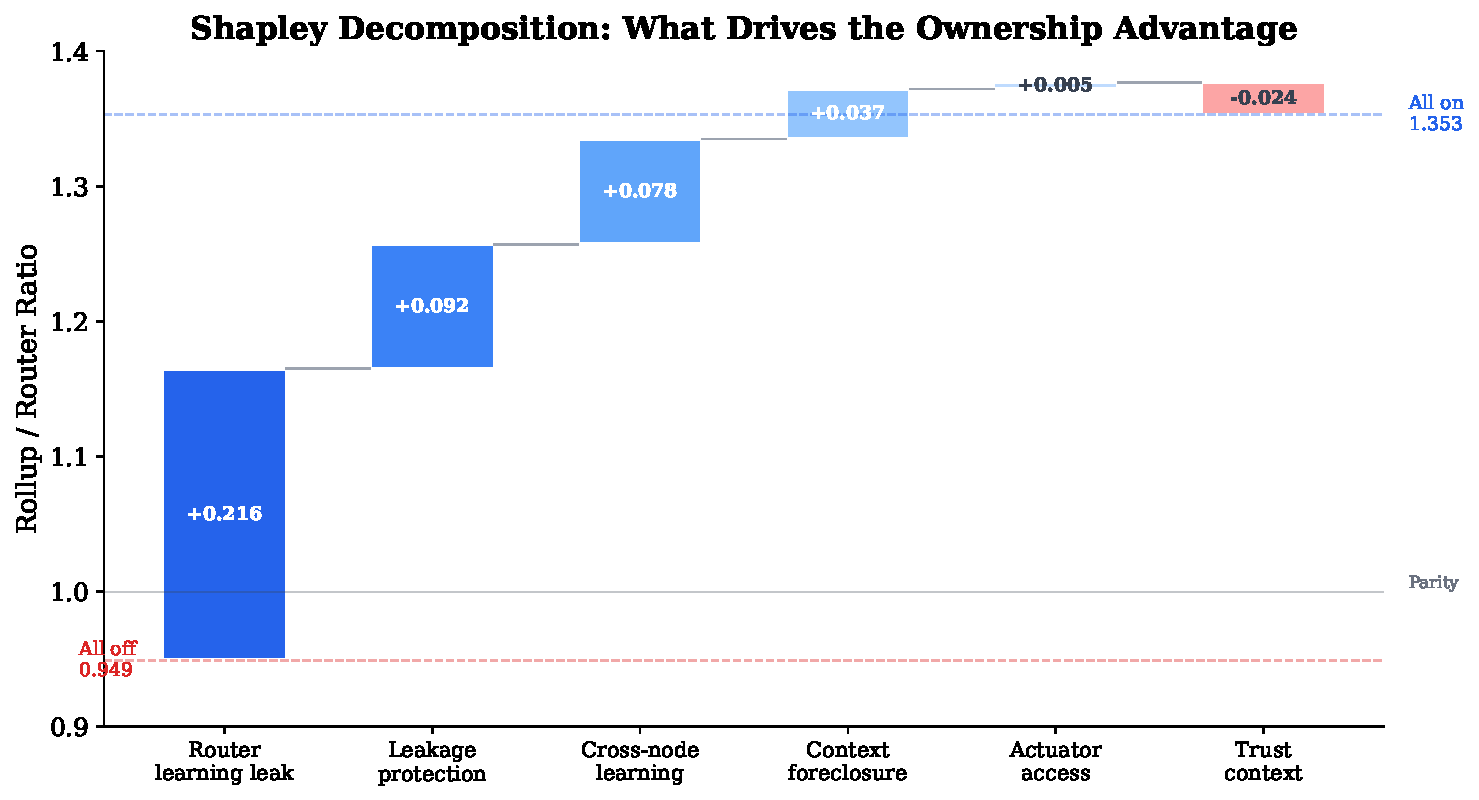
\includegraphics[width=\textwidth]{fig_shapley.pdf}
\caption{Shapley value decomposition of the rollup/router surplus ratio (seed 42; see Table~\ref{tab:shapley} for 5-seed mean $\pm$ std). Router learning leakage is the dominant channel. Note: the foreclosure bar is positive in this seed but negative on average across seeds---see text.}
\label{fig:shapley}
\end{figure}

\subsection{Regime Boundaries}
\label{sec:boundaries}

The baseline is one point in parameter space. Here we trace the boundaries by sweeping each parameter family. Ownership density (fraction of the graph the rollup owns, with acquisition disabled): when the rollup owns only 10\% of nodes, ownership costs exceed the information benefit and the rollup loses to the router. As density increases to 90\%, the rollup advantage grows to 9.2\% over the router, because more internal interactions mean more leakage protection and richer cross-node learning. Ownership cost: the rollup wins at every tested level (0.00--0.30 per node per step), maintaining a 26\% net advantage at the highest overhead. Visibility spread: even at the most favorable visibility for the router ($\nu_{\text{rtr}} = 0.50$, $\nu_{\text{int}} = 0.40$, spread of 0.10), the rollup still wins by $\sim$20\%, because router learning leakage and cross-node learning operate independently of the visibility spread.

\textbf{Router learning leakage ($\lambda_R$).} This is the paper's core empirical question, not a settled parameter. $\lambda_R$ governs how aggressively platforms extract and redistribute client operational intelligence---and the entire quantitative story flows downstream from it. We do not claim to know the true value. We claim that the \textit{ranking} of institutional forms is robust across all tested values, while the \textit{magnitude} is an empirical question that specific industries must answer. Table~\ref{tab:lr_sensitivity} presents the full sensitivity:

\begin{table}[H]
\centering
\caption{Rollup/Router ratio vs.\ router learning leakage rate $\lambda_R$ (5 seeds each). This is the most important table in the paper: it shows where the thesis is strong, where it thins, and where it reduces to a slim structural margin.}
\label{tab:lr_sensitivity}
\begin{tabular}{rrr}
\toprule
$\lambda_R$ & Mean ratio & Interpretation \\
\midrule
0.00 & 1.035 & No learning leakage: rollup barely wins \\
0.05 & 1.110 & Mild leakage \\
0.10 & 1.167 & Moderate leakage \\
0.15 & 1.274 & Baseline \\
0.20 & 1.371 & Strong leakage \\
0.30 & 1.615 & Very strong leakage \\
\bottomrule
\end{tabular}
\end{table}

\noindent At $\lambda_R = 0$, the rollup still wins (ratio 1.035) through leakage protection and cross-node learning alone, but the advantage is slim enough that modest agency costs could reverse it. At $\lambda_R = 0.15$ (baseline), the advantage is 26\%. The framework does not resolve which industries sit where on this axis---that is the empirical question it poses. The observed pattern of enterprise AI clients restricting data use (Harvey in legal, Epic in healthcare) suggests that firms believe $\lambda_R > 0$ in their industries, which is evidence for the thesis but not proof of the specific magnitude.

\subsection{Data-Isolated Router}
\label{sec:isolated}

The data-isolated router tests the platform's best response: what if the router contractually prevents cross-client data use, eliminating the dominant Shapley channel? The isolated router has the same visibility and interaction parameters as the standard router but charges a per-node subscription fee ($c_{\text{sub}}$ per node per step) instead of extracting learning leakage.

In the baseline, the isolated router generates net surplus of 1,646---13\% above the standard router (1,455) but 12\% below the rollup (1,860). A subscription cost sweep reveals the crossover: the isolated router beats the standard router at every tested subscription cost up to $c_{\text{sub}} = 0.15$ per node per step, where the two converge. Beyond this, the subscription fee outweighs the benefit of data isolation.

The isolated router's leakage cost (0.426 per event) is \textit{lower than the market's} (0.500), because the market exposes interactions at full visibility ($\nu = 1.0$) while the isolated router shields them ($\nu = 0.85$). The ranking market $>$ isolated router for leakage cost means that the isolated router is a genuinely better platform design---but it cannot match the rollup because the rollup also benefits from cross-node learning ($+0.071$ Shapley) and leakage protection ($+0.051$ Shapley) that no platform arrangement can replicate.

This result has a practical implication: firms like Harvey AI that contractually restrict data use are implementing the isolated router. They outperform standard SaaS platforms---but they cannot replicate the ownership advantage. The gap between the isolated router and the rollup represents the irreducible value of common ownership.

\subsection{Superlinearity Without Complementarity}
\label{sec:superlinearity}

With the complementarity coefficient set to zero (the $\kappa_{ij}$ term in Eq.~\ref{eq:match} contributes nothing), the baseline produces a superlinearity ratio of 2.07 (single-seed, seed 42): the combined portfolio generates 107\% more surplus than the sum of its halves. This number requires careful interpretation. Most of the effect is a \textit{network-size} property: splitting 12 nodes into two groups of 6 and measuring each separately excludes all coordination between the groups (36 cross-group pairs out of 66 total). Any network where value comes from connections between nodes would show a similar ratio---this component is not ownership-specific.

The ownership-specific component is layered on top: those cross-group pairs get internal visibility ($\nu = 0.1$) instead of market visibility, so each new coordination opportunity created by combining the groups is also a \textit{higher-quality} opportunity than it would be under separate ownership. The conglomerate premium is real, but it is primarily the claim that each additional node creates new coordination opportunities with every existing node---and that common ownership makes those opportunities more valuable per interaction than they would be in the market.

\subsection{Competing Dynamics}
\label{sec:competing}

The parallel-world design cleanly attributes performance differences to institutional form. But it systematically understates the rollup's advantage because it does not model competitive dynamics. In the competing-world simulation, all four forms coexist in a single economy: the rollup starts with 3 nodes, the remaining 27 are split equally among router clients, isolated router clients, and market participants (9 each). Each acquisition \textit{actually removes} the node from its prior regime.

\begin{table}[H]
\centering
\caption{Competing-World Results (50 steps, 30 nodes, passive router, seed 42)}
\label{tab:competing}
\begin{tabular}{lrrrrrr}
\toprule
Regime & Gross & Own.\ cost & Sub.\ cost & Net & Events & Nodes (final) \\
\midrule
Market & 200 & 0 & 0 & 200 & 103 & 9 \\
Router & 283 & 0 & 0 & 283 & 130 & 4 \\
Iso.\ Router & 257 & 0 & 11 & 246 & 149 & 5 \\
Rollup & 495 & 75 & 0 & 420 & 148 & 12 \\
\bottomrule
\end{tabular}
\end{table}

The rollup's net surplus ($420$) exceeds the router's ($283$) by 48\%, the isolated router's ($246$) by 71\%, and the market's ($200$) by $2.1\times$. The rollup acquires 12 of 30 nodes. Across 10 seeds, the rollup wins in all 10 with mean surplus $385$ vs.\ the router's $202$.

\textbf{Router response strategies.} We test two progressively stronger responses, each applied \textit{preemptively from step 0} across 10 seeds:

\begin{itemize}[leftmargin=*]
\item \textbf{Preemptive data isolation}: the router eliminates learning leakage ($\lambda_R = 0$) from the first step. Result: mean rollup surplus $385$, router $202$---the rollup still wins 10/10. Eliminating the dominant channel preemptively does not overcome the remaining ownership-contingent channels.

\item \textbf{Full defensive}: the router eliminates learning leakage \textit{and} doubles trust investment from step 0. Result: mean rollup surplus $385$, router $202$---virtually identical to isolation alone. Doubling trust investment adds almost nothing, confirming that trust is the wrong channel (Shapley $-0.011$).
\end{itemize}

\noindent The router's strongest available move---preemptive data isolation, addressing the dominant channel before any competitive damage---narrows the gap from 1.91$\times$ to 1.90$\times$. The residual advantage is entirely from ownership-contingent channels (cross-node learning, internal visibility) that no platform strategy can address, because they require owning the nodes, not just serving them differently.

\subsection{Industry Predictions}
\label{sec:industries}

We calibrate the framework to all 35 services verticals from \citet{sequoia2025services}, setting each vertical's durability, specificity, and transferability based on the industry characteristics described above. Table~\ref{tab:industries} reports the full results, grouped by the Sequoia quadrant.

\begin{table}[p]
\centering
\caption{Services Taxonomy: Predicted Rollup Advantage by Industry (3-seed mean $\pm$ std). Industries from \citet{sequoia2025services}, grouped by quadrant. D$\times$S$\times$T = durability $\times$ specificity $\times$ transferability (H/M/L). Shading intensity reflects advantage magnitude.}
\label{tab:industries}
\vspace{-4pt}
{\footnotesize
\renewcommand{\arraystretch}{0.92}
\begin{tabular}{llclr}
\toprule
Industry & TAM & D$\times$S$\times$T & Quadrant & Rollup/Router \\
\midrule
Cybersecurity & \$30B+ & H$\times$H$\times$M & Watch & \cellcolor{green!28} $1.276 \pm .044$ \\
Pharmacy back-office & \$30B+ & M$\times$M$\times$H & Next wave & \cellcolor{green!24} $1.263 \pm .039$ \\
KYC / AML & \$30--50B & H$\times$H$\times$M & Autopilot & \cellcolor{green!22} $1.258 \pm .041$ \\
Claims adjusting & \$50--80B & M$\times$M$\times$H & Autopilot & \cellcolor{green!21} $1.255 \pm .039$ \\
Mortgage origination & \$30--50B & M$\times$M$\times$H & Autopilot & \cellcolor{green!21} $1.255 \pm .039$ \\
Medical admin & \$20B+ & M$\times$M$\times$H & Next wave & \cellcolor{green!21} $1.255 \pm .039$ \\
Supply chain \& procurement & \$200B+ & H$\times$H$\times$M & Next wave & \cellcolor{green!21} $1.254 \pm .041$ \\
Accounting \& audit & \$50--80B & H$\times$H$\times$M & Autopilot & \cellcolor{green!20} $1.251 \pm .042$ \\
Clinical trials / CRO & \$80B+ & H$\times$H$\times$M & Watch & \cellcolor{green!20} $1.251 \pm .042$ \\
ERP implementation & \$50B+ & H$\times$H$\times$M & Watch & \cellcolor{green!20} $1.251 \pm .040$ \\
Freight brokerage & \$100B+ & L$\times$M$\times$H & Watch & \cellcolor{green!19} $1.248 \pm .040$ \\
Insurance brokerage & \$140--200B & M$\times$M$\times$H & Autopilot & \cellcolor{green!18} $1.247 \pm .040$ \\
Real estate closing & \$20--25B & M$\times$M$\times$H & Autopilot & \cellcolor{green!18} $1.245 \pm .040$ \\
SEO / SEM & \$50B+ & L$\times$M$\times$H & Watch & \cellcolor{green!18} $1.245 \pm .040$ \\
Recruitment \& staffing & \$200B+ & M$\times$M$\times$H & Watch & \cellcolor{green!18} $1.245 \pm .040$ \\
Cost estimation & \$16B & M$\times$M$\times$M & Autopilot & \cellcolor{green!17} $1.244 \pm .038$ \\
Market research & \$45B & M$\times$M$\times$M & Watch & \cellcolor{green!17} $1.244 \pm .038$ \\
Tax advisory & \$30--35B & H$\times$H$\times$L & Autopilot & \cellcolor{green!17} $1.242 \pm .044$ \\
Healthcare rev cycle & \$50--80B & M$\times$L$\times$H & Autopilot & \cellcolor{green!17} $1.241 \pm .040$ \\
Payroll \& compliance & \$50--70B & M$\times$L$\times$H & Autopilot & \cellcolor{green!16} $1.238 \pm .039$ \\
Architecture & \$25B+ & M$\times$M$\times$M & Watch & \cellcolor{green!15} $1.237 \pm .039$ \\
Paralegal / LPO & \$36B & H$\times$H$\times$L & Autopilot & \cellcolor{green!15} $1.236 \pm .042$ \\
PR \& comms & \$20B+ & M$\times$M$\times$M & Copilot & \cellcolor{green!15} $1.235 \pm .038$ \\
Management consulting & \$300B+ & H$\times$H$\times$L & Copilot & \cellcolor{green!14} $1.234 \pm .043$ \\
Wealth mgmt ops & \$30B+ & H$\times$H$\times$L & Next wave & \cellcolor{green!14} $1.234 \pm .043$ \\
Advertising & \$100B+ & L$\times$M$\times$H & Watch & \cellcolor{green!14} $1.233 \pm .039$ \\
Fund administration & \$15--20B & H$\times$H$\times$L & Next wave & \cellcolor{green!14} $1.233 \pm .043$ \\
Legal, transactional & \$20--25B & H$\times$H$\times$L & Autopilot & \cellcolor{green!12} $1.228 \pm .037$ \\
Executive search & \$20B+ & H$\times$H$\times$L & Copilot & \cellcolor{green!12} $1.228 \pm .042$ \\
Patent / IP & \$15--20B & H$\times$H$\times$L & Watch & \cellcolor{green!12} $1.228 \pm .037$ \\
Graphic / UX design & \$30B+ & L$\times$L$\times$H & Copilot & \cellcolor{green!11} $1.223 \pm .039$ \\
IT managed services & \$100B+ & L$\times$L$\times$H & Autopilot & \cellcolor{green!9} $1.219 \pm .039$ \\
Corporate training & \$50B+ & L$\times$L$\times$H & Watch & \cellcolor{green!9} $1.219 \pm .039$ \\
Admin assistants & \$80B+ & L$\times$L$\times$H & Watch & \cellcolor{green!8} $1.215 \pm .038$ \\
Travel management & \$15B+ & L$\times$L$\times$H & Watch & \cellcolor{green!8} $1.215 \pm .038$ \\
\bottomrule
\end{tabular}
}
\end{table}

Three patterns emerge. First, the rollup dominates in \textit{every} tested vertical---the advantage ranges from 21.5\% (travel, admin) to 27.6\% (cybersecurity). The mechanism is universal; only the magnitude is industry-specific.

Second, the advantage is driven by the \textit{interaction} of durability and transferability, not by either alone. The highest-scoring industry is cybersecurity (1.28$\times$)---not because it has the most durable context (legal and patent/IP have higher $\rho_L$), but because it combines high durability with moderate transferability. A zero-day discovered at one portfolio company protects all others; an incident response playbook developed for one client improves response across the portfolio. Pure durability without transferability (legal transactional, patent/IP: 1.23$\times$) scores lower because cross-node learning---the second-largest Shapley channel---is weak when each engagement is too bespoke for operational patterns to transfer. The bottom of the table---travel, admin, IT services (1.22$\times$)---consists of verticals where context expires quickly and carries little competitive value.

\textbf{These are testable predictions.} The framework predicts that AI-driven consolidation should appear earliest in high-$\rho_L$, high-$\ell$ verticals and be weakest in low-$\rho_L$, low-$\ell$ verticals. The $\lambda_R$ boundary condition adds a further prediction: in verticals where platforms can credibly commit to data isolation ($\lambda_R \to 0$), the rollup advantage narrows to $\sim$3.5\%. Enterprise AI providers offering strict data isolation (Harvey in legal) are implementing the isolated router---addressing the dominant channel but unable to replicate the cross-node learning and internal visibility that ownership provides.

\begin{remark}[Applying the Framework to Your Industry]
The framework requires three inputs to generate a prediction for any industry:
\begin{enumerate}[leftmargin=*]
\item \textbf{Durability} ($\rho_L$): If a competitor learned your most sensitive operational detail today, how long could they exploit it? Years (legal strategy, tax positions, security architecture) $\to$ $\rho_L > 0.8$. Months (pricing, staffing patterns) $\to$ $0.4$--$0.7$. Days or weeks (patch status, booking data) $\to$ $\rho_L < 0.3$.

\item \textbf{Specificity} ($\ell$): How much competitive damage does revealing context on a single coordination cause? High if the interaction exposes proprietary strategy (financial audits, M\&A diligence) $\to$ $\ell = 0.5$--$0.95$. Low if the interaction is routine and standardized (IT provisioning, payroll) $\to$ $\ell = 0.05$--$0.3$.

\item \textbf{Transferability} ($\tau$): Does operational knowledge at one firm improve operations at another? High if the work is standardized across firms (medical coding, insurance forms) $\to$ $\tau > 0.03$. Low if each engagement is bespoke (litigation strategy, executive coaching) $\to$ $\tau < 0.01$.
\end{enumerate}
\noindent Set these three parameters and run the simulation to see where your industry falls. Transferability also predicts the optimal AI architecture for the rollup: if $\tau$ is high, operational patterns generalize across the portfolio and fine-tuning a model on proprietary portco data compounds---the model \textit{learns} your operations. If $\tau$ is low, each engagement is too bespoke for patterns to transfer through model weights; use a generalist model with rich operational context provided at inference instead. The replication code is available at the repository listed on the title page.
\end{remark}

%=============================================================================
\section{Discussion}
%=============================================================================

\subsection{Reinterpreting the Coasean Singularity}

The Coasean singularity thesis---that AI-driven transaction cost reduction will dissolve firms into agent-mediated markets---captures one real channel while missing two others. Yes, AI reduces the cost of market coordination. But simultaneously, platform intermediation may \textit{amplify} information leakage (the dominant channel in our Shapley decomposition), and ownership enables cross-node learning that market coordination cannot replicate. The net effect on firm boundaries depends on the magnitude of these countervailing forces.

Our results suggest a conditional revision: if the router learning leakage hypothesis holds (and real-world practices like Harvey AI's data restrictions suggest firms believe it does), it is the dominant channel driving ownership advantage, producing $1.9\times$ the leakage cost of the open market ($0.93$ vs.\ $0.50$ per event). The data-isolated router recovers most of the gap but cannot match the rollup, because ownership captures channels that no contractual arrangement can replicate.

The updated Coasean logic: \textit{in AI-intensive industries with local, leakage-sensitive context, intermediation may not reduce information frictions but amplify them.} The firm exists not to reduce transaction costs but to prevent the extraction and redistribution of its scarce context. The firm does not just persist; it expands because each acquisition marginally improves its information position relative to competitors. This is the cybernetic arbitrage: the spread between the market's valuation of assets as isolated operations and their actual value as nodes in an AI-coordinated portfolio---a spread that is small per-node but cumulative across the vertical.

\subsection{Autopilots Are Routers}

A growing thesis in venture capital holds that AI-native services companies---``autopilots'' that sell the \textit{work} rather than the \textit{tool}---will capture the \$6 of services spend for every \$1 of software spend \citep{sequoia2025services}. The argument: every improvement in the underlying model makes the autopilot faster and cheaper, compounding a data advantage from doing the work at scale. Autopilots are projected to dominate outsourced, intelligence-heavy verticals first (insurance brokerage, healthcare billing, tax compliance) and expand toward judgement-heavy work as AI matures.

Our framework reveals a structural tension in this thesis. \textbf{The autopilot is a more capable router, but a router nonetheless.} When Harvey drafts an NDA, it intermediates the coordination between client and counterparty. When Anterior processes a prior authorization, it intermediates between provider and payer. The autopilot \textit{does} the work, but it does not \textit{own} the node where context is born. It sees the client's operational data---exception patterns, pricing sensitivity, negotiation positions---and this creates the same information economics our model formalizes:

\begin{itemize}[leftmargin=*]
\item If the autopilot uses client data to improve its service for \textit{all} clients, it is a standard router with learning leakage. Each client's operational intelligence is ingested, systematized, and deployed to serve competitors.

\item If the autopilot commits to data isolation (per-client model weights, contractual data restrictions), it is our isolated router: better than the standard platform, but unable to capture the cross-node learning and internal visibility channels that ownership provides.
\end{itemize}

\noindent The driving effect is strategic: the context owner knows that revealing information to an external party is costly, so they rationally withhold. When a law firm hires Harvey to draft an NDA, sharing its full negotiation strategy would produce a better draft---but it also exposes that strategy to an entity the firm does not control. The firm faces the revelation-leakage tradeoff and, in our simulation, chooses partial revelation in $\sim$20\% of such interactions. Worse drafts, worse coordination, less surplus. When the rollup's own subsidiary drafts the NDA, the firm faces no such tradeoff: internal visibility is low ($\nu = 0.1$), so full revelation is cheap, and the rollup reveals freely in 88\% of events. The ownership advantage is not that the rollup has better technology---it is that firms are willing to reveal more to an entity they own than to one they hire.

The prediction is not that autopilots will fail---they will likely outperform copilots and general SaaS platforms, exactly as \citet{sequoia2025services} argues. The prediction is that autopilots face the same structural ceiling as any intermediary: they can eliminate the learning leakage channel through data isolation, but they cannot replicate the cross-node learning, internal visibility, and competitive foreclosure that ownership provides. In verticals where these channels matter (legal, tax, accounting, cybersecurity---the top of Table~\ref{tab:industries}), the endgame is not the autopilot but the entity that owns the firms the autopilot serves. The autopilot is the wedge; the rollup is the moat.

\subsection{Where the Framework Predicts Rollup Dominance---and Where It Does Not}

The regime map and industry calibrations (Section~\ref{sec:industries}) generate testable predictions about where different institutional forms should dominate:

\begin{enumerate}[leftmargin=*]
\item \textbf{The rollup wins where context is durable and specific} ($\rho_L > 0.7$, high $\ell$). Legal transactional work, tax advisory, and specialized financial services occupy this region. These verticals should see AI-driven consolidation first.

\item \textbf{The data-isolated router wins where platforms can credibly commit to isolation}. When $\lambda_R \to 0$ (through contractual restriction or technical architecture), the rollup advantage narrows to $\sim$3.5\%. If ownership costs are also high (agency costs, regulatory overhead), the isolated router can dominate. This predicts that platforms committing to data isolation---contractually guaranteeing that one client's operational data will not be used to serve another---should outperform platforms that pool client data across their user base.

\item \textbf{The router/market wins where context is short-lived and non-specific} ($\rho_L < 0.3$, low $\ell$). IT managed services, commodity logistics, and contexts where information is too ephemeral to exploit. Here, leakage protection contributes little, and the platform's breadth advantage in learning from standardized, transferable patterns may offset the rollup's ownership channels.

\item \textbf{The rollup thesis fails when cross-node learning is absent}. If operations are too heterogeneous for knowledge to transfer across portfolio companies ($\tau \to 0$), or if AI cannot extract transferable patterns, the second-largest channel disappears. Combined with data isolation ($\lambda_R = 0$), this leaves only leakage protection---a $\sim$5\% advantage that may not justify ownership overhead.
\end{enumerate}

\noindent The framework does not predict a universal answer. It maps parameter space to institutional form dominance, generating industry-specific predictions that can be tested against observed patterns of AI-era consolidation.

\subsection{Implications for Industrial Organization}

Three implications follow from the framework that are worth stating explicitly.

\textbf{Cross-node learning has increasing returns.} The transfer bonus in the model scales with the number of distinct verticals in the owned portfolio ($\tau \cdot |\{v_k\}| / K$). This creates a positive feedback loop: more nodes owned $\to$ more verticals covered $\to$ richer cross-node learning $\to$ higher acquisition value of the next node $\to$ more nodes owned. The first entity to reach critical mass in a vertical has a compounding advantage that late entrants cannot overcome, because they face a cold-start problem: they cannot match the cross-node learning without the nodes, and they cannot justify acquiring the nodes without the learning. This implies that AI-era consolidation, once it begins in a vertical, should exhibit winner-take-most dynamics---not because of demand-side network effects (as in platform markets) but because of supply-side learning economies that are structurally ownership-contingent.

\textbf{Operational access can approximate ownership for information flows.} The model treats ownership as binary: a node is owned or it is not. In practice, deep operational engagement---consulting, advisory, integration work---can provide signal quality approaching ownership levels without requiring financial acquisition. A firm embedded inside a company for twelve weeks, observing workflows and exception handling at full depth, achieves something close to the rollup's internal visibility ($\sigma_{\text{own}} = 0.9$) without taking an equity position. This suggests the rollup's information advantage can be partially achieved through services relationships, with financial acquisition reserved for nodes where the context is durable enough to justify the ownership overhead. The consulting engagement becomes the sensing layer; the acquisition follows only where the learning compounds.

\textbf{The parameter space determines whether platforms evolve toward ownership.} The framework predicts not just which regime dominates, but whether the platform-to-ownership transition occurs at all. Where context is durable and specific (high $\rho_L$, high $\ell$---legal, tax, cybersecurity), the leakage cost per unit is high enough that rational actors withhold from intermediaries, degrading the platform's data quality and pushing it toward ownership as the only reliable path to full context access. The historical analogue is Metropolis, a parking technology company that could not sell its software to parking garage operators and instead acquired the garages themselves.

But where context is ephemeral and non-specific (low $\rho_L$, low $\ell$---advertising, logistics, commodity transactions), the platform model can be stable \textit{even with full learning leakage}. Meta's advertising platform extracts retailer conversion data through installed tracking pixels and uses it to optimize ad delivery for all advertisers, including each retailer's competitors. Retailers accept this because the data is high-volume but low-value-per-unit: no individual retailer's conversion events constitute a durable competitive asset, and the value of Meta's ad optimization exceeds the leakage cost. This is the standard router in our model---but operating in the region of parameter space where the rollup advantage is smallest ($\sim$1.22$\times$) and the leakage cost is low enough that clients rationally participate.

The implication is that the autopilot-to-ownership transition is industry-dependent. In the top of Table~\ref{tab:industries}, it is the likely equilibrium: the autopilot is the wedge, but ownership is the moat. In the bottom, the platform model persists because there is not enough durable, specific context to justify the overhead of ownership---and not enough leakage cost to drive clients away.

\textbf{Model training as a new form of cross-node learning.} As AI labs seek operational data for model improvement---through instrumentation partnerships, screen observation, and workflow capture---a question arises: does the model itself absorb the cross-node learning channel? If a lab has trained on 10,000 dental practices across 50 portfolios, the model already knows the optimal scheduling approach. The rollup's ability to observe its own five practices and transfer learnings adds nothing the model does not already provide. In this view, cross-node learning ($\sim$23\% of the Shapley effect) is partially commoditized by model training: the ``what works at dental practices'' knowledge becomes embedded in the model and available to everyone, not just the owner.

The rollup's remaining advantage shifts from \textit{learning what works} (which the model increasingly provides) to \textit{knowing what is happening right now and having the authority to act on it}. The model knows general patterns from historical training data. The rollup knows that this specific practice's lead hygienist quit yesterday, that the local competitor just closed, that the insurance contract is up for renegotiation next month. These are real-time, firm-specific observations that training pipelines cannot capture at the same latency---and that require ownership-level visibility ($\nu = 0.1$) to observe at all. The rollup's advantage migrates from pattern recognition to operational latency and actuator access.

The emerging structure of lab-PE partnerships is consistent with this analysis. Labs are pursuing joint ventures with portfolio owners rather than commercial API relationships---seeking ownership-equivalent context access through equity alignment. This implicitly validates the framework's prediction: commercial access does not provide the context depth that ownership does, and the labs are reaching for ownership-like structures to close the gap.

\subsection{Limitations}

While we model ownership costs (overhead and integration friction), we do not model \textit{agency costs}---and agency costs may be the binding constraint on the rollup thesis. Each subsidiary's management has its own incentives---empire-building, risk aversion, headcount padding---that diverge from the parent company's goal. \citet{berger1995} found that diversified firms trade at a 13--15\% discount to the sum of their parts, and \citet{jensen1986} attributes this largely to inefficient internal capital allocation. Our flat ownership cost ($c_{\text{overhead}}$ per node per step) understates this problem: real agency costs are likely \textit{convex} in portfolio size. At the baseline rollup advantage of $\sim$26\%, convex agency costs could plausibly eliminate the margin.

The deeper issue is that context access and context \textit{compounding} are not the same thing. A large consulting firm like BCG or McKinsey has had deep operational access to thousands of companies over decades---arguably more ``context born at the node'' than any rollup could accumulate. Yet this context does not compound: it lives in slide decks, in partners' heads, in institutional memory that walks out the door with departing staff. The organizational structure of a consulting firm---partner incentives misaligned with firm-wide knowledge management, practice areas operating semi-independently, no central system of record for operational observations---is itself an agency cost that prevents the conversion of contact into structured, reusable intelligence. Our model assumes that the rollup can convert ownership into a central, compounding intelligence layer. Whether this assumption holds depends on whether AI-enabled coordination can reduce the organizational overhead of multi-node management sufficiently to overcome the agency costs that have historically made conglomerates value-destructive. This is the strongest version of the counterargument to our thesis, and the model does not resolve it.

Additional limitations in brief: the model uses scalar policy quality rather than heterogeneous policies across nodes; the parallel-world structural advantage is scale-invariant (ratio 1.23 at 200 nodes, 1.22 at 1000 nodes) but the competing-world tipping dynamic requires sufficient simulation duration to accumulate critical ownership density; the model does not capture strategic information withholding by router clients, though firms like Harvey already implement such restrictions in practice; and ownership is treated as a per-node property rather than a structural one---the model does not capture vertical completion effects (monopoly pricing power, complete sector information) that would accrue from owning every firm in a sector.

%=============================================================================
\section{Conclusion}
%=============================================================================

This paper develops a framework that maps the parameter space of information economics to institutional form dominance, comparing four forms---fragmented markets, platform routers, data-isolated routers, and cybernetic rollups---over a directed graph economy. The framework identifies three mechanisms driving ownership advantage (router learning leakage, cross-node learning, leakage protection), establishes their ranking as stable across calibrations, and generates testable predictions about which industries should see AI-driven consolidation.

The central finding is that ownership advantage is robust but not universal. The rollup dominates in verticals where context is durable and specific---legal transactional work, tax advisory, specialized financial services. The advantage narrows where context is short-lived (IT managed services: 1.22$\times$) and nearly vanishes where platforms can credibly commit to data isolation and cross-node learning is absent. A data-isolated router---the platform's best response---eliminates the dominant channel but cannot replicate the cross-node learning and internal visibility that ownership provides, trailing the rollup by $\sim$12\% at baseline calibration.

For theory, the contribution is the framework itself: a mapping from parameter space to institutional form dominance that identifies which mechanisms matter, in what order, and under what conditions. For practice, it generates predictions: AI-driven consolidation should appear earliest in high-durability, high-specificity verticals (legal, tax, specialized finance); platform providers should invest in credible data isolation; and firms using SaaS platforms for operationally sensitive coordination should understand that each interaction may train a model that serves their competitors.

The cybernetic arbitrage is the spread between the market's valuation of assets as isolated operations and their actual value as nodes in an AI-coordinated portfolio where context is internalized rather than leaked. Where that spread exists---and this paper maps where it should---ownership captures the value that AI creates.

%=============================================================================
% Bibliography
%=============================================================================

\bibliographystyle{aer}

\begin{thebibliography}{99}

\bibitem[Agrawal et~al.(2018)]{agrawal2018}
Agrawal, Ajay, Joshua Gans, and Avi Goldfarb. 2018. ``Prediction Machines: The Simple Economics of Artificial Intelligence.'' \textit{Harvard Business Review Press}.

\bibitem[Armstrong(2006)]{armstrong2006}
Armstrong, Mark. 2006. ``Competition in Two-Sided Markets.'' \textit{RAND Journal of Economics} 37(3): 668--691.

\bibitem[Benzell and Brynjolfsson(2024)]{benzell2024}
Benzell, Seth G., and Erik Brynjolfsson. 2024. ``AI and the Boundary of the Firm.'' Working paper.

\bibitem[Bonatti et~al.(2022)]{bonatti2022}
Bonatti, Alessandro, Munther Dahleh, Thibaut Horel, and Amir Nouripour. 2022. ``Selling Information in Competitive Environments.'' arXiv:2202.08780.

\bibitem[Berger and Ofek(1995)]{berger1995}
Berger, Philip G., and Eli Ofek. 1995. ``Diversification's Effect on Firm Value.'' \textit{Journal of Financial Economics} 37(1): 39--65.

\bibitem[Brynjolfsson and Mitchell(2017)]{brynjolfsson2017}
Brynjolfsson, Erik, and Tom Mitchell. 2017. ``What Can Machine Learning Do? Workforce Implications.'' \textit{Science} 358(6370): 1530--1534.

\bibitem[Christensen(1997)]{christensen1997}
Christensen, Clayton M. 1997. \textit{The Innovator's Dilemma}. Boston: Harvard Business School Press.

\bibitem[Chopra et~al.(2024)]{chopra2024}
Chopra, Ayush, et~al. 2024. ``What Can We Learn from a Billion Agents?'' arXiv:2501.10025.

\bibitem[Coase(1937)]{coase1937}
Coase, Ronald H. 1937. ``The Nature of the Firm.'' \textit{Economica} 4(16): 386--405.

\bibitem[Danco(2017)]{danco2017}
Danco, Alex. 2017. ``Understanding Abundance.'' \textit{Social Capital}, February.

\bibitem[Grossman and Hart(1986)]{grossman1986}
Grossman, Sanford J., and Oliver D. Hart. 1986. ``The Costs and Benefits of Ownership: A Theory of Vertical and Lateral Integration.'' \textit{Journal of Political Economy} 94(4): 691--719.

\bibitem[Hart and Moore(1990)]{hart1990}
Hart, Oliver, and John Moore. 1990. ``Property Rights and the Nature of the Firm.'' \textit{Journal of Political Economy} 98(6): 1119--1158.

\bibitem[Hart(1995)]{hart1995}
Hart, Oliver. 1995. \textit{Firms, Contracts, and Financial Structure}. Oxford: Clarendon Press.

\bibitem[Hobart(2024)]{hobart2024routers}
Hobart, Byrne. 2024. ``Routers, Apps, AGI.'' \textit{The Diff}, October.

\bibitem[Jensen(1986)]{jensen1986}
Jensen, Michael C. 1986. ``Agency Costs of Free Cash Flow, Corporate Finance, and Takeovers.'' \textit{American Economic Review} 76(2): 323--329.

\bibitem[Lang and Stulz(1994)]{lang1994}
Lang, Larry H.P., and Ren\'{e} M. Stulz. 1994. ``Tobin's q, Corporate Diversification, and Firm Performance.'' \textit{Journal of Political Economy} 102(6): 1248--1280.

\bibitem[Larson(2025)]{larson2025cybernetic}
Larson, Soren. 2025. ``Cybernetic Arbitrage: AI is Inverting Aggregation Theory.'' \textit{hypersoren.xyz}, December.

\bibitem[Parker et~al.(2016)]{parker2016}
Parker, Geoffrey G., Marshall W. Van Alstyne, and Sangeet Paul Choudary. 2016. \textit{Platform Revolution}. New York: W.W. Norton.

\bibitem[Azhar(2024)]{azhar2024}
Azhar, Azeem. 2024. ``From ChatGPT to a Billion Agents.'' \textit{Exponential View}, December.

\bibitem[Shapiro(2024)]{shapiro2024}
Shapiro, David. 2024. ``Billions of Agents.'' September.

\bibitem[Toma\v{s}ev et~al.(2025)]{tomasev2025}
Toma\v{s}ev, Nenad, Matija Franklin, Joel Z. Leibo, Julian Jacobs, William A. Cunningham, Iason Gabriel, and Simon Osindero. 2025. ``Virtual Agent Economies.'' arXiv:2509.10147.

\bibitem[Bek(2026)]{sequoia2025services}
Bek, Julien. 2026. ``Services: The New Software.'' \textit{Sequoia Capital}, March.

\bibitem[Shahidi et~al.(2025)]{shahidi2025}
Shahidi, Peyman, Gili Rusak, Benjamin S. Manning, Andrey Fradkin, and John J. Horton. 2025. ``The Coasean Singularity? Demand, Supply, and Market Design with AI Agents.'' NBER Working Paper.

\bibitem[Rochet and Tirole(2003)]{rochet2003}
Rochet, Jean-Charles, and Jean Tirole. 2003. ``Platform Competition in Two-Sided Markets.'' \textit{Journal of the European Economic Association} 1(4): 990--1029.

\bibitem[Williamson(1975)]{williamson1975}
Williamson, Oliver E. 1975. \textit{Markets and Hierarchies: Analysis and Antitrust Implications}. New York: Free Press.

\bibitem[Williamson(1985)]{williamson1985}
Williamson, Oliver E. 1985. \textit{The Economic Institutions of Capitalism}. New York: Free Press.

\end{thebibliography}

\end{document}
